\documentclass[12pt, a4paper, oneside]{ctexart}
\usepackage{amsmath, amsthm, amssymb, bm, color, framed, graphicx, hyperref, mathrsfs, mathtools, enumerate, tikz}
\usepackage{float}
\usepackage{booktabs}
\usepackage{subcaption} 



\usetikzlibrary{patterns}

\title{\textbf{Homework 11}}
\author{萃英学院\qquad 2022级\qquad 王一鑫}
\date{\today}
\linespread{1.5}
\newcounter{problemname}
\newenvironment{problem}{\begin{framed}\stepcounter{problemname}\par\noindent\textsc{Problem \arabic{problemname}. }}{\end{framed}\par}
\newenvironment{solution}{%
	\par\noindent\textsc{Solution. }\ignorespaces
}{%
	\hfill$\qed$\par
}
\newenvironment{note}{\par\noindent\textsc{Note of Problem \arabic{problemname}. }}{\\\par}

\begin{document}
	
	\maketitle
	
	
	\begin{problem}
		(Exercise 5.41)
		Let \( G \) be a simple graph with an odd number of vertices. Prove that if \( G \) is regular of degree \( \Delta \), then 
		\[
		\chi'(G) = \Delta + 1.
		\]
		
	\end{problem}
	
	\begin{solution}
		Since \( G \) is regular of degree \( \Delta \), the number of edges in \( G \) is
		\[
		|E| = \frac{\Delta |V|}{2}.
		\]
		Let \( |V| = 2m + 1 \) be odd, where \( m \in \mathbb{N} \). Then
		\[
		|E| = \frac{\Delta(2m + 1)}{2}.
		\]
		
		We consider an edge coloring \( c : E \to \{1, \dots, k\} \) using \( k \) colors. Assume for contradiction that \( \chi'(G) \leq \Delta \), i.e., that \( G \) is properly edge-colorable with at most \( \Delta \) colors.
		
		Then the total number of edges is partitioned among \( k \leq \Delta \) color classes. By the pigeonhole principle, there exists at least one color used on at least
		\[
		\left\lceil \frac{|E|}{k} \right\rceil \geq \left\lceil \frac{\Delta(2m + 1)/2}{\Delta} \right\rceil = \left\lceil \frac{2m + 1}{2} \right\rceil = m + 1
		\]
		edges.
		
		Therefore, at least one color class contains \( m + 1 \) edges. But \( G \) has only \( 2m + 1 \) vertices, and each color class must consist of pairwise non-adjacent edges (i.e., a matching). The maximum size of a matching in a graph with \( 2m + 1 \) vertices is at most \( m \), since each edge uses two distinct vertices. Hence, a matching with \( m + 1 \) edges must involve at least \( 2(m + 1) = 2m + 2 > 2m + 1 \) vertices, which is impossible.
		
		This contradiction implies that \( G \) cannot be properly edge-colored using only \( \Delta \) colors. Thus, we must have \( \chi'(G) \geq \Delta + 1 \).
		
		On the other hand, Vizing's Theorem tells us that for any simple graph,
		\[
		\chi'(G) \leq \Delta + 1.
		\]
		Therefore, we conclude that \( \chi'(G) = \Delta + 1 \).
	\end{solution}
	
	\begin{problem}
		(Exercise 6.5)
		
		Prove that, if \( G = G(V_1, V_2) \) is a bipartite graph in which the degree of each vertex in \( V_1 \) 
		is not less than the degree of each vertex in \( V_2 \), then \( G \) has a complete matching.
	\end{problem}
	
	\begin{solution}
		Let \( \varphi(A) \subseteq V_2 \) denote the set of neighbors of a subset \( A \subseteq V_1 \), i.e., those vertices in \( V_2 \) adjacent to at least one vertex in \( A \). According to Corollary 6.2, a complete matching from \( V_1 \) to \( V_2 \) exists if and only if
		\[
		|A| \leq |\varphi(A)|
		\quad \text{for all subsets } A \subseteq V_1.
		\]
		
		We will prove this condition holds under the hypothesis that all vertices in \( V_1 \) have degree at least as large as those in \( V_2 \).
		
		Suppose, for the sake of contradiction, that there exists a subset \( A \subseteq V_1 \) such that \( |A| > |\varphi(A)| \). Let \( B = \varphi(A) \subseteq V_2 \). Consider the number of edges between \( A \) and \( B \). We count these edges in two ways:
		
		On one hand, since each vertex in \( A \) has degree at least \( d_1 \), and all its neighbors are in \( B \), the total number of edges from \( A \) to \( B \) is at least
		\[
		e(A, B) \geq |A| \cdot d_1.
		\]
		
		On the other hand, since the degree of every vertex in \( V_2 \) is at most \( d_2 \leq d_1 \), the total number of edges from \( B \) to \( A \) is at most
		\[
		e(A, B) \leq |B| \cdot d_2.
		\]
		
		Combining these, we obtain:
		\[
		|A| \cdot d_1 \leq |B| \cdot d_2.
		\]
		Since \( d_1 \geq d_2 \), this implies \( |A| \leq |B| = |\varphi(A)| \), contradicting our assumption that \( |A| > |\varphi(A)| \).
		
		Therefore, for all \( A \subseteq V_1 \), it must hold that \( |A| \leq |\varphi(A)| \). By Corollary 6.2, this implies that a complete matching from \( V_1 \) to \( V_2 \) exists.
	\end{solution}
	
	\begin{problem}
		(Exercise 6.7)
	
	Decide which of the following families of subsets of \( E = \{G, R, A, P, H, S\} \) have transversals, 
	find a transversal for those that have them, and list all the partial transversals 
	of those that have no transversal:
	\begin{enumerate}[(i)]
		\item \( (\{R\}, \{R,G\}, \{A,G\}, \{A,R\}) \)
		\item \( (\{G,R\}, \{R,P,H\}, \{G,S\}, \{R,H\}) \)
	\end{enumerate}
		
	\end{problem}
	
	\begin{solution} 
		
		\begin{enumerate}[(i)]
			\item No trasversal.
			
			We now list all possible partial transversals: $\emptyset$, $\{R\}$, $\{G\}$, $\{A\}$, $\{R, G\}$, $\{R, A\}$, $\{G, R\}$, $\{G, R, A\}$.
			
			\item Transversal:
			 \( \{G, P, S, H\} \).
		\end{enumerate}
		
	\end{solution}
	
	\begin{problem}
		(Exercise 6.9)
		
		Let \( E \) be the set \( \{1, 2, \ldots, 50\} \). How many different transversals has the family
		\[
		(\{1,2\}, \{2,3\}, \{3,4\}, \ldots, \{50,1\})?
		\]
	\end{problem}
	
	\begin{solution}
		
		There is only one transversal - namely, $\{1,2,\cdots,50\}$.
		
	\end{solution}
	
	\begin{problem}
		(Exercise 6.14)
		
		Verify Theorems 6.5 and 6.6 for the Petersen graph in the two cases:
		\begin{enumerate}
			\item when \( v \) and \( w \) are adjacent vertices;
			\item when \( v \) and \( w \) are not adjacent.
		\end{enumerate}
		
	\end{problem}
	
	\begin{solution}
		
		\begin{enumerate}[(i)]
			\item For this case, we verify Theorem 6.5 by counting the maximum number of edge-disjoint paths connecting two distinct adjacent vertices $v$ and $w$ of a connected graph and the minimum number of edges in a $vw$-disconnecting set. See Figure \eqref{fig:thm6.5}.
			\begin{figure}[H]
				\small
				\centering
				.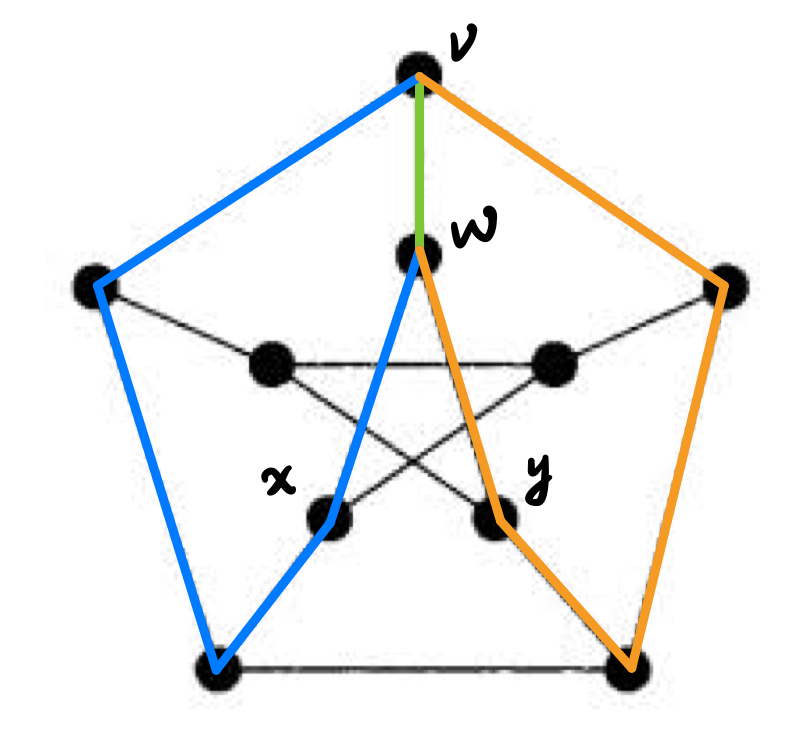
\includegraphics[width=0.36\columnwidth]{Figure/fig1.jpg}
				\caption{Edge-disjoint paths of the Petersen Graph}
				\label{fig:thm6.5}
			\end{figure}
			We know from the figure that there are three edge-disjoint paths which are coloured green, blue and orange respectively, and $E = \{vw, xw, yw\}$ is a $vw$-disconnecting set. Thus Theorem 6.5 holds.
			\item See Figure \eqref{fig:thm6.6}.
			\begin{figure}[H]
				\small
				\centering
				.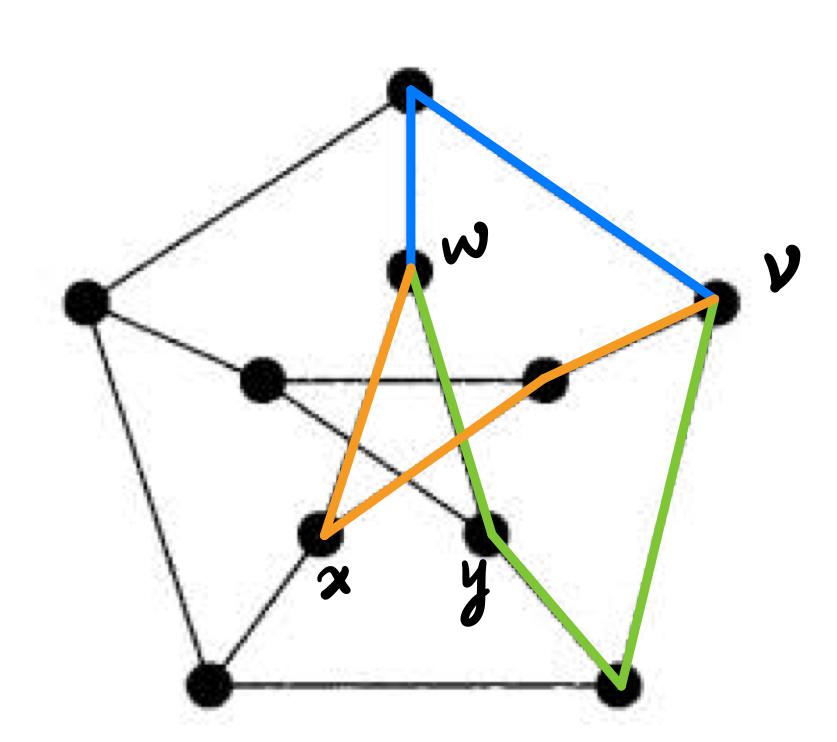
\includegraphics[width=0.36\columnwidth]{Figure/fig2.jpg}
				\caption{Edge-disjoint paths of the Petersen Graph}
				\label{fig:thm6.6}
			\end{figure}
			We know from the figure that there are three vertex-disjoint paths which are coloured green, blue and orange respectively, and $V = \{w, x, y\}$ is a $vw$-separating set. Thus Theorem 6.6 holds.
		\end{enumerate}
		
	\end{solution}
	
	
	
	
	\begin{problem}
	
		 Compute the number of different perfect matchings of complete bipartite graph $K_{n,n}$ and complete graph $K_{2n}$.
		
		
	\end{problem}
	
	\begin{solution}
		\begin{enumerate}[(i)]
			\item 			
			To count the number of perfect matchings in \( K_{n,n} \), we proceed as follows. Each perfect matching corresponds to a bijection \( f: X \to Y \), where each vertex \( x_i \in X \) is matched with a distinct vertex \( y_j \in Y \). Since there are \( n! \) such bijections from an \( n \)-element set to another \( n \)-element set, the number of perfect matchings in \( K_{n,n} \) is exactly
			\[
			M_{n,n} = n!
			\]
			
			\item Let $K_{2n}$ denote the complete graph on $2n$ vertices. We aim to compute the number of perfect matchings in $K_{2n}$, denoted by $M_{2n}$.
			
			To form a perfect matching, we begin by choosing a pair of vertices from the $2n$ available. The number of ways to choose the first vertex is $2n$, and the number of ways to choose its partner is $2n - 1$. After forming this pair, we have $2n - 2$ vertices remaining. We then select a vertex from these and pair it with one of the remaining $2n - 3$ vertices, and so on. Proceeding in this way, we construct $n$ pairs, and the number of such ordered selections is:
			\[
			(2n - 1)(2n - 3)(2n - 5)\cdots 1
			\]
			This is $(2n-1)!!$.
			
			
		\end{enumerate}
		
		
	\end{solution}
	
	
	
\end{document}


